
Das Programm basiert auf dem \textbf{Model-View-ViewModel (MVVM)}-Pattern, welches eine klare Trennung zwischen Benutzeroberfläche (View), Präsentationslogik (ViewModel) und Datenmodell (Model) gewährleistet. Diese Architektur ist in WPF-Anwendungen weit verbreitet und fördert die Wartbarkeit, Testbarkeit sowie Erweiterbarkeit der Software.

\subsubsection*{Aufbau der Anwendung}

Die Anwendung gliedert sich in drei zentrale Komponenten:

\begin{itemize}
    \item \textbf{Model:} \\
    Die Model-Schicht beinhaltet die zentralen Datenklassen wie \texttt{User}, \texttt{Role}, \texttt{UserRole}, \texttt{CleanupLog} sowie \texttt{AppConfig}. Sie spiegeln die Datenbankstruktur wider und sind mittels Entity Framework Core mit der zugrunde liegenden Datenbank verbunden.
    
    \item \textbf{ViewModel:} \\
    Die ViewModels enthalten die Anwendungslogik sowie Bindings zu den Views. Dazu gehören Properties, Commands und Methoden. Zentrale Klassen sind u.\,a.:
    \begin{itemize}
        \item \texttt{NavigationVM} – steuert den Seitenwechsel
        \item \texttt{LoginVM}, \texttt{RegisterVM} – enthalten die Authentifizierungslogik
        \item \texttt{HomeVM}, \texttt{CleanupVM}, \texttt{SettingsVM}, \texttt{InformationVM}, \texttt{AdministrationVM} – zuständig für die jeweilige Seitenlogik
    \end{itemize}
    
    \item \textbf{View:} \\
    Die Views werden in XAML definiert und über \texttt{DataTemplates} im \texttt{App.xaml}-Ressourcendictionary an ihre zugehörigen ViewModels gebunden:

\begin{figure}[H]
    \centering
    \begin{xamlcode}
<DataTemplate DataType="{x:Type vm:HomeVM}">
    <view:Home />
</DataTemplate>
\end{xamlcode}
    \caption{DataTemplate für die View-Bindung von HomeVM}
\end{figure}
% \begin{figure}[H]
%     \centering
%     \includegraphics[width=0.85\textwidth]{src/datatemp_code.png}
%     \caption{DataTemplate für die View-Bindung von HomeVM}
% \end{figure}

    Durch diese Bindung wird beim Wechsel der Eigenschaft \texttt{CurrentView} automatisch die zugehörige View angezeigt.
\end{itemize}

\subsubsection*{Navigation}

Die Navigation wird zentral im \texttt{NavigationVM} gesteuert. Dieses besitzt die Property \texttt{CurrentView}, die während der Laufzeit dynamisch auf das gewünschte ViewModel gesetzt wird. Die Navigation erfolgt über \texttt{RelayCommands}, die den Seitenwechsel auslösen:

\begin{figure}[H]
    \centering
    \begin{cs}
private void Home(object obj) => CurrentView = new HomeVM();
private void Cleanup(object obj) => CurrentView = new CleanupVM();
private void Settings(object obj) => CurrentView = new SettingsVM();
private void Information(object obj) => CurrentView = new InformationVM();
private void Administration(object obj) => CurrentView = new AdministrationVM();

public NavigationVM()
{
    HomeCommand = new RelayCommand(Home);
    CleanupCommand = new RelayCommand(Cleanup);
    SettingsCommand = new RelayCommand(Settings);
    InformationCommand = new RelayCommand(Information);
    AdministrationCommand = new RelayCommand(Administration);
    LogoutCommand = new RelayCommand(Logout);

    CurrentView = new HomeVM();
}
\end{cs}

    \caption{Command-Implementierung für Navigation}
\end{figure}
% \begin{figure}[H]
%     \centering
%     \includegraphics[width=0.85\textwidth]{src/navigation_code.png}
%     \caption{Command-Implementierung für Navigation}
% \end{figure}

Im \texttt{MainWindow.xaml} wird ein \texttt{ContentControl} verwendet, das stets den aktuellen Inhalt anhand der Property \texttt{CurrentView} darstellt:

\begin{figure}[H]
    \centering
    \begin{xamlcode}
<Grid Grid.Column="1" HorizontalAlignment="Stretch" VerticalAlignment="Stretch">
    <ContentControl x:Name="Pages" Content="{Binding CurrentView}" />
</Grid>
\end{xamlcode}
    \caption{ContentControl für dynamische View-Anzeige}
\end{figure}
% \begin{figure}[H]
%     \centering
%     \includegraphics[width=0.85\textwidth]{src/contentControl_code.png}
%     \caption{ContentControl für dynamische View-Anzeige}
% \end{figure}

Ein \texttt{AdminVisibilityConverter} regelt die Sichtbarkeit bestimmter Bereiche – etwa des Administrationsmenüs – abhängig von der Benutzerrolle.

\subsubsection*{Command-Handling mit \texttt{RelayCommand}}

Zur Umsetzung der Benutzerinteraktionen – wie z.\,B. Button-Klicks zur Navigation – nutzt die Anwendung das \texttt{RelayCommand}-Pattern. Dabei handelt es sich um eine flexible Implementierung des \texttt{ICommand}-Interfaces. Sie erlaubt es, Logik direkt im ViewModel zu definieren, ohne Code-Behind-Dateien zu verwenden.

\texttt{RelayCommand} kapselt dabei eine Aktion (\texttt{Action<object>}) und eine optionale Bedingung zur Ausführbarkeit (\texttt{Func<object, bool>}).

\begin{figure}[H]
    \centering
    \begin{cs}
class RelayCommand : ICommand
{
    private readonly Action<object> _execute;
    private readonly Func<object, bool> _canExecute;

    public event EventHandler CanExecuteChanged
    {
        add { CommandManager.RequerySuggested += value; }
        remove { CommandManager.RequerySuggested -= value; }
    }
    public RelayCommand(Action<object> execute, Func<object, bool> canExecute = null)
    {
        _execute = execute;
        _canExecute = canExecute;
    }
    public bool CanExecute(object parameter) => _canExecute == null || _canExecute(parameter);
    public void Execute(object parameter) => _execute(parameter);
}
\end{cs}
    \caption{Grundstruktur eines RelayCommands}
\end{figure}
% \begin{figure}[H]
%     \centering
%     \includegraphics[width=0.85\textwidth]{src/relayCommand_code.png}
%     \caption{Grundstruktur eines RelayCommands}
% \end{figure}

Diese Trennung fördert die Wiederverwendbarkeit und testbare Logik, was das MVVM-Muster ideal ergänzt.

\subsubsection*{Property-Änderungen mit \texttt{ViewModelBase}}

Alle ViewModels erben von \texttt{ViewModelBase}, welche die Schnittstelle \texttt{INotifyPropertyChanged} implementiert. Diese sorgt dafür, dass Änderungen an Eigenschaften automatisch an die View gemeldet werden. Ein zentrales Prinzip von Data Binding in WPF.

\begin{figure}[H]
    \centering
    \begin{cs}
public class ViewModelBase : INotifyPropertyChanged
{
    public event PropertyChangedEventHandler PropertyChanged;
    public void OnPropertyChanged([CallerMemberName] string propName = null)
    {
        PropertyChanged?.Invoke(this, new PropertyChangedEventArgs(propName));
    }
}
\end{cs}
    \caption{PropertyChanged-Implementierung}
\end{figure}
% \begin{figure}[H]
%     \centering
%     \includegraphics[width=0.85\textwidth]{src/viewModelBase_code.png}
%     \caption{PropertyChanged-Implementierung}
% \end{figure}

\subsubsection*{Architekturübersicht}

Die folgende Grafik zeigt das vereinfachte Klassendiagramm der Anwendung und veranschaulicht das Zusammenspiel zwischen View, ViewModel und Model gemäß dem MVVM-Muster:

\begin{figure}[H]
    \centering
    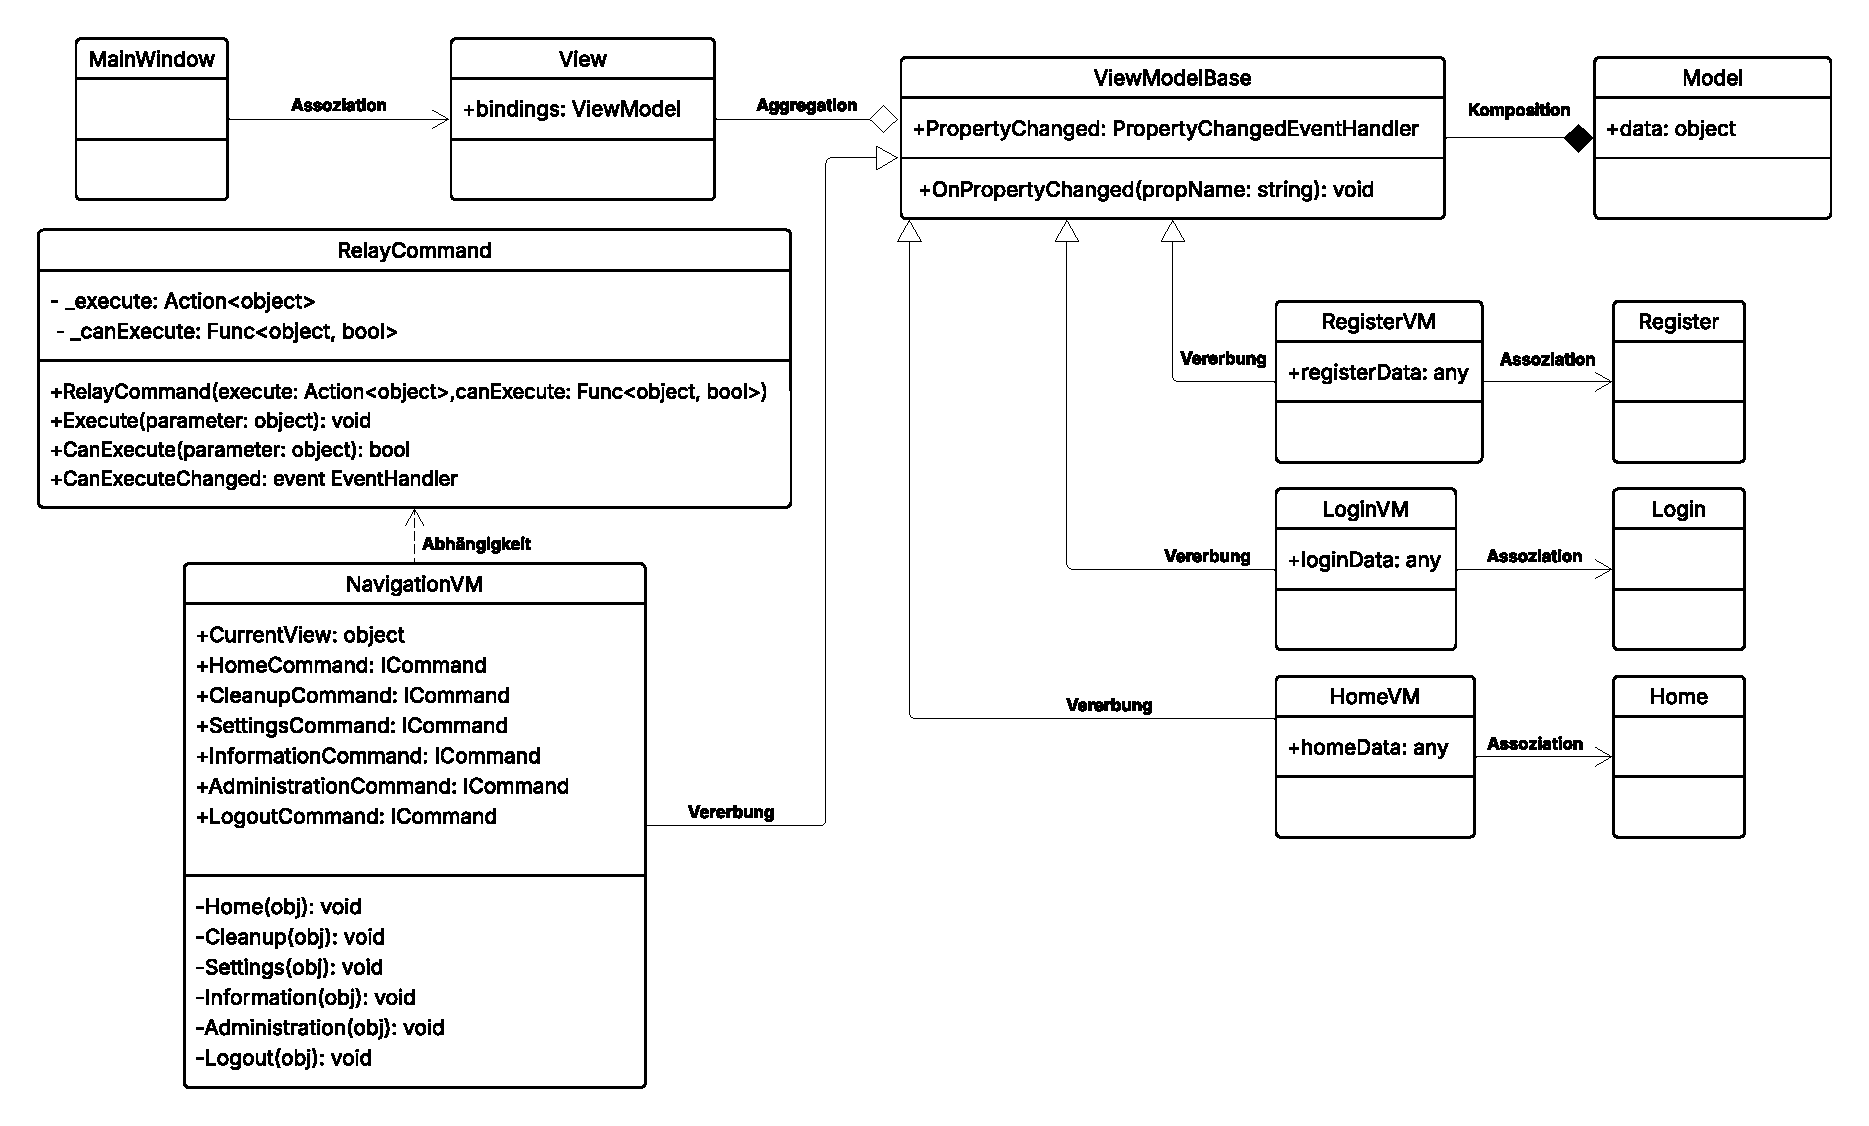
\includegraphics[width=1\textwidth]{src/klassen_diagramm.pdf}
    \caption{Architekturübersicht des Garbage-Collection-Tools (MVVM)}
\end{figure}

